% Options for packages loaded elsewhere
\PassOptionsToPackage{unicode}{hyperref}
\PassOptionsToPackage{hyphens}{url}
\PassOptionsToPackage{dvipsnames,svgnames,x11names}{xcolor}
%
\documentclass[
  letterpaper,
]{article}

\usepackage{amsmath,amssymb}
\usepackage{iftex}
\ifPDFTeX
  \usepackage[T1]{fontenc}
  \usepackage[utf8]{inputenc}
  \usepackage{textcomp} % provide euro and other symbols
\else % if luatex or xetex
  \usepackage{unicode-math}
  \defaultfontfeatures{Scale=MatchLowercase}
  \defaultfontfeatures[\rmfamily]{Ligatures=TeX,Scale=1}
\fi
\usepackage{lmodern}
\ifPDFTeX\else  
    % xetex/luatex font selection
\fi
% Use upquote if available, for straight quotes in verbatim environments
\IfFileExists{upquote.sty}{\usepackage{upquote}}{}
\IfFileExists{microtype.sty}{% use microtype if available
  \usepackage[]{microtype}
  \UseMicrotypeSet[protrusion]{basicmath} % disable protrusion for tt fonts
}{}
\makeatletter
\@ifundefined{KOMAClassName}{% if non-KOMA class
  \IfFileExists{parskip.sty}{%
    \usepackage{parskip}
  }{% else
    \setlength{\parindent}{0pt}
    \setlength{\parskip}{6pt plus 2pt minus 1pt}}
}{% if KOMA class
  \KOMAoptions{parskip=half}}
\makeatother
\usepackage{xcolor}
\usepackage[top=20mm,bottom=25mm,left=20mm,right=20mm,heightrounded]{geometry}
\setlength{\emergencystretch}{3em} % prevent overfull lines
\setcounter{secnumdepth}{-\maxdimen} % remove section numbering
% Make \paragraph and \subparagraph free-standing
\makeatletter
\ifx\paragraph\undefined\else
  \let\oldparagraph\paragraph
  \renewcommand{\paragraph}{
    \@ifstar
      \xxxParagraphStar
      \xxxParagraphNoStar
  }
  \newcommand{\xxxParagraphStar}[1]{\oldparagraph*{#1}\mbox{}}
  \newcommand{\xxxParagraphNoStar}[1]{\oldparagraph{#1}\mbox{}}
\fi
\ifx\subparagraph\undefined\else
  \let\oldsubparagraph\subparagraph
  \renewcommand{\subparagraph}{
    \@ifstar
      \xxxSubParagraphStar
      \xxxSubParagraphNoStar
  }
  \newcommand{\xxxSubParagraphStar}[1]{\oldsubparagraph*{#1}\mbox{}}
  \newcommand{\xxxSubParagraphNoStar}[1]{\oldsubparagraph{#1}\mbox{}}
\fi
\makeatother


\providecommand{\tightlist}{%
  \setlength{\itemsep}{0pt}\setlength{\parskip}{0pt}}\usepackage{longtable,booktabs,array}
\usepackage{calc} % for calculating minipage widths
% Correct order of tables after \paragraph or \subparagraph
\usepackage{etoolbox}
\makeatletter
\patchcmd\longtable{\par}{\if@noskipsec\mbox{}\fi\par}{}{}
\makeatother
% Allow footnotes in longtable head/foot
\IfFileExists{footnotehyper.sty}{\usepackage{footnotehyper}}{\usepackage{footnote}}
\makesavenoteenv{longtable}
\usepackage{graphicx}
\makeatletter
\newsavebox\pandoc@box
\newcommand*\pandocbounded[1]{% scales image to fit in text height/width
  \sbox\pandoc@box{#1}%
  \Gscale@div\@tempa{\textheight}{\dimexpr\ht\pandoc@box+\dp\pandoc@box\relax}%
  \Gscale@div\@tempb{\linewidth}{\wd\pandoc@box}%
  \ifdim\@tempb\p@<\@tempa\p@\let\@tempa\@tempb\fi% select the smaller of both
  \ifdim\@tempa\p@<\p@\scalebox{\@tempa}{\usebox\pandoc@box}%
  \else\usebox{\pandoc@box}%
  \fi%
}
% Set default figure placement to htbp
\def\fps@figure{htbp}
\makeatother

\makeatletter
\@ifpackageloaded{tcolorbox}{}{\usepackage[skins,breakable]{tcolorbox}}
\@ifpackageloaded{fontawesome5}{}{\usepackage{fontawesome5}}
\definecolor{quarto-callout-color}{HTML}{909090}
\definecolor{quarto-callout-note-color}{HTML}{0758E5}
\definecolor{quarto-callout-important-color}{HTML}{CC1914}
\definecolor{quarto-callout-warning-color}{HTML}{EB9113}
\definecolor{quarto-callout-tip-color}{HTML}{00A047}
\definecolor{quarto-callout-caution-color}{HTML}{FC5300}
\definecolor{quarto-callout-color-frame}{HTML}{acacac}
\definecolor{quarto-callout-note-color-frame}{HTML}{4582ec}
\definecolor{quarto-callout-important-color-frame}{HTML}{d9534f}
\definecolor{quarto-callout-warning-color-frame}{HTML}{f0ad4e}
\definecolor{quarto-callout-tip-color-frame}{HTML}{02b875}
\definecolor{quarto-callout-caution-color-frame}{HTML}{fd7e14}
\makeatother
\makeatletter
\@ifpackageloaded{caption}{}{\usepackage{caption}}
\AtBeginDocument{%
\ifdefined\contentsname
  \renewcommand*\contentsname{Table of contents}
\else
  \newcommand\contentsname{Table of contents}
\fi
\ifdefined\listfigurename
  \renewcommand*\listfigurename{List of Figures}
\else
  \newcommand\listfigurename{List of Figures}
\fi
\ifdefined\listtablename
  \renewcommand*\listtablename{List of Tables}
\else
  \newcommand\listtablename{List of Tables}
\fi
\ifdefined\figurename
  \renewcommand*\figurename{Figure}
\else
  \newcommand\figurename{Figure}
\fi
\ifdefined\tablename
  \renewcommand*\tablename{Table}
\else
  \newcommand\tablename{Table}
\fi
}
\@ifpackageloaded{float}{}{\usepackage{float}}
\floatstyle{ruled}
\@ifundefined{c@chapter}{\newfloat{codelisting}{h}{lop}}{\newfloat{codelisting}{h}{lop}[chapter]}
\floatname{codelisting}{Listing}
\newcommand*\listoflistings{\listof{codelisting}{List of Listings}}
\makeatother
\makeatletter
\makeatother
\makeatletter
\@ifpackageloaded{caption}{}{\usepackage{caption}}
\@ifpackageloaded{subcaption}{}{\usepackage{subcaption}}
\makeatother

\usepackage{bookmark}

\IfFileExists{xurl.sty}{\usepackage{xurl}}{} % add URL line breaks if available
\urlstyle{same} % disable monospaced font for URLs
\hypersetup{
  colorlinks=true,
  linkcolor={blue},
  filecolor={Maroon},
  citecolor={Blue},
  urlcolor={blue},
  pdfcreator={LaTeX via pandoc}}


\title{COMM 3710: Intro to Quantitative Research\\
COMM 3711: \textbf{(HON)} Intro to Quantitative Research}
\usepackage{etoolbox}
\makeatletter
\providecommand{\subtitle}[1]{% add subtitle to \maketitle
  \apptocmd{\@title}{\par {\large #1 \par}}{}{}
}
\makeatother
\subtitle{Lecture: Mondays (9:40 - 11:35 am), BEH S 111\\
Lab: Wednesdays (9:40 - 11:35 am), BEH S 111\\
\strut \\
Professor: Dr.~Sara K. Yeo\\
Email: \href{mailto:sara.yeo@utah.edu}{\nolinkurl{sara.yeo@utah.edu}}\\
Office Hours:
\href{https://outlook.office.com/bookwithme/user/98f1ac91631e47eb9f502658b45494f9@umail.utah.edu/meetingtype/SVRwCe7HMUGxuT6WGxi68g2?bookingcode=6a99b2dc-526d-4185-8078-0f5a72d23764&anonymous&ismsaljsauthenabled&ep=mlink}{By
appointment}}
\author{}
\date{}

\begin{document}
\maketitle


\section{Course Outline}\label{sec-outline}

This course is a basic research methods course for those with little or
no experience or course work in quantitative communication research.
COMM 3710 is a quantitative intensive (QI) course. The goal of this
course is to provide you with a critical framework for evaluating social
science research and some hands-on experience in the process of
conducting empirical investigations.

Key topics include:

\begin{itemize}
\tightlist
\item
  Developing a question into a research project
\item
  Formalizing hypotheses and research questions grounded in theory
\item
  Testing hypotheses and research questions
\item
  Conceptual and operational definitions
\item
  Measurement, sampling, and research design
\item
  Data analysis in communication research
\item
  Interpreting research results
\item
  Communicating research
\item
  \textbf{(HON)} Improve presentation skills
\item
  \textbf{(HON)} Identify a research question and propose a research
  study
\item
  \textbf{(HON)} Connect the concepts and skills learned in this course
  to a potential Honors thesis
\end{itemize}

\begin{tcolorbox}[enhanced jigsaw, breakable, coltitle=black, opacityback=0, rightrule=.15mm, colframe=quarto-callout-note-color-frame, bottomtitle=1mm, opacitybacktitle=0.6, bottomrule=.15mm, left=2mm, toptitle=1mm, titlerule=0mm, title=\textcolor{quarto-callout-note-color}{\faInfo}\hspace{0.5em}{Note}, colback=white, arc=.35mm, toprule=.15mm, leftrule=.75mm, colbacktitle=quarto-callout-note-color!10!white]

You are expected to log into the course Canvas website regularly
(\textbf{at least 3-5 times per week}), complete and submit work on
time, and ask questions if you need help. \textbf{It is your
responsibility as a student to ask questions in a timely manner during
scheduled labs and office hours, if you need help.}

\end{tcolorbox}

\section{Required Text and Readings}\label{sec-text}

The textbook for this course is listed below and available online. The
course fee that you paid when you enrolled covers Inclusive Access to
the Wrench textbook via Canvas. Additional readings will be provided as
PDF documents on Canvas.

Wrench, J.S. (2019) \emph{Quantitative Research Methods for
Communication: A Hands-On Approach} (4th edition). New York, NY: Oxford
University Press.

\begin{itemize}
\tightlist
\item
  To access this textbook, navigate to your \textbf{Bookshelf} on the
  Canvas site for this course.
\item
  This textbook is available through the
  \href{https://www.campusstore.utah.edu/inclusiveaccess/}{Inclusive
  Access program}, which provides you with digital access to the
  textbook via Canvas at a reduced price.
\item
  You may opt out of the Inclusive Access program
  \href{https://www.campusstore.utah.edu/inclusiveaccess/}{here}.
  However, the textbook is \textbf{required}, and you are expected to
  have it, even if you opt out of this program.
\end{itemize}

\section{Technology Requirements}\label{sec-tech}

To ensure that you have full access to the course, you will need:

\begin{itemize}
\item
  Reliable access to a laptop or desktop computer. A mobile device
  (tablet, phone) is not sufficient to complete this course. Please
  bring a laptop to lab.
\item
  An Internet browser compatible with
  \href{https://utah.instructure.com/}{Canvas}. For more information,
  see this
  \href{https://community.canvaslms.com/docs/DOC-10720-67952720329}{page}.
  Announcements, assignments, readings, etc., will be posted there. You
  should be familiar with Canvas. If you need help with Canvas, visit
  the \href{https://community.canvaslms.com/docs/DOC-10701}{Canvas
  Getting Started Guide for Students}.
\item
  We will be using \href{https://www.r-project.org/}{R} in lab for data
  analysis. You do not need to have this set up before the semester
  begins. We will get set up in lab at the beginning of the semester.
\item
  Additionally, access to a text-editor (e.g., Wordpad, TextEdit,
  Notepad++, Atom), Microsoft Office (Word, Excel, PowerPoint), and
  Adobe Acrobat (free for UofU students) are recommended.
\end{itemize}

\begin{tcolorbox}[enhanced jigsaw, breakable, coltitle=black, opacityback=0, rightrule=.15mm, colframe=quarto-callout-note-color-frame, bottomtitle=1mm, opacitybacktitle=0.6, bottomrule=.15mm, left=2mm, toptitle=1mm, titlerule=0mm, title=\textcolor{quarto-callout-note-color}{\faInfo}\hspace{0.5em}{Note}, colback=white, arc=.35mm, toprule=.15mm, leftrule=.75mm, colbacktitle=quarto-callout-note-color!10!white]

You are expected to know how to take a screenshot with your computer. A
photo of your laptop or computer screen taken with your mobile device is
\emph{not} a screenshot.

\end{tcolorbox}

\section{Course Requirements}\label{sec-requirements}

Course grades will be based on the following:

\begin{itemize}
\tightlist
\item
  Quizzes (110 pts)
\item
  Attendance (28 pts)
\item
  Lab assignments (125 pts)
\item
  Lab presentations (50 pts)
\item
  \textbf{(HON)} Article presentation (50 pts)
\item
  \textbf{(HON)} Research proposal (50 pts)
\end{itemize}

\subsection{Quizzes}\label{quizzes}

Weekly quizzes will be administered online via Canvas. All quizzes will
be based on assigned readings. \textbf{No make-up or late quizzes be
administered}. You can take the quiz at any time during the week it is
assigned. Quizzes are each worth 10 points. Note that quizzes are timed
and you will only have \textbf{one attempt} at each quiz--please do not
start a quiz unless you are ready to complete it.

\begin{tcolorbox}[enhanced jigsaw, breakable, coltitle=black, opacityback=0, rightrule=.15mm, colframe=quarto-callout-important-color-frame, bottomtitle=1mm, opacitybacktitle=0.6, bottomrule=.15mm, left=2mm, toptitle=1mm, titlerule=0mm, title=\textcolor{quarto-callout-important-color}{\faExclamation}\hspace{0.5em}{Important}, colback=white, arc=.35mm, toprule=.15mm, leftrule=.75mm, colbacktitle=quarto-callout-important-color!10!white]

Quizzes will open on Tuesday at 12:00 am and are due on Sunday of that
week at 11:59 pm.

\end{tcolorbox}

\subsection{Attendance}\label{attendance}

Attendance is required for lectures and labs. Out of respect for your
instructor and peers, please arrive on time to classes.

\subsection{Lab Assignments}\label{lab-assignments}

There are 9 lab assignments. Information on individual assignments will
be provided in lab and on Canvas. Assignment due dates will be listed on
Canvas. Please pay attention to any changes in the due dates on Canvas.

\textbf{Late assignments will not be accepted}.

\subsection{Lab Presentations}\label{lab-presentations}

Each student will give one (1) presentation in lab as part of a team.
More information and detailed instructions will be provided during lab.

\subsection{\texorpdfstring{\textbf{(HON)} Article
Presentation}{(HON) Article Presentation}}\label{hon-article-presentation}

Each student will present and lead a class discussion about one assigned
reading. Students are required to have an individual meeting with
Prof.~Yeo \textbf{before their presentation} to receive feedback. More
information and guidelines will be provided separately.

\subsection{\texorpdfstring{\textbf{(HON)} Research
Proposal}{(HON) Research Proposal}}\label{hon-research-proposal}

Each student will formulate a research question and propose a study
using the concepts and skills learned in the course. The research
proposal should be at least 10 pages (12-point font, 1-in margins,
double-spaced). \textbf{The draft of the proposal will be due in Week
10.} Students are encouraged to meet with Prof.~Yeo individually as they
work on their proposal. Students are \textbf{required} to meet with
Prof.~Yeo to receive feedback on their draft. The revised, final
proposal is due at the end of the course. More information and
guidelines will be provided separately.

\section{Course Grading}\label{course-grading}

\begin{tcolorbox}[enhanced jigsaw, breakable, coltitle=black, opacityback=0, rightrule=.15mm, colframe=quarto-callout-important-color-frame, bottomtitle=1mm, opacitybacktitle=0.6, bottomrule=.15mm, left=2mm, toptitle=1mm, titlerule=0mm, title=\textcolor{quarto-callout-important-color}{\faExclamation}\hspace{0.5em}{Important}, colback=white, arc=.35mm, toprule=.15mm, leftrule=.75mm, colbacktitle=quarto-callout-important-color!10!white]

If you wish to dispute your grade on any assignment or quiz, you must
put your concerns in writing (please adhere to the
\hyperref[sec-policies]{course email policy}) to your
\hyperref[sec-ta]{graduate teaching assistant}, clearly outlining your
rationale. These concerns must be presented to your TA within one week
of receiving your grade.

\end{tcolorbox}

Grades in this course will be based on the following scale.

\begin{longtable}[]{@{}lc@{}}
\toprule\noalign{}
Grade & Score (\%) \\
\midrule\noalign{}
\endhead
\bottomrule\noalign{}
\endlastfoot
A & 93 to 100 \\
A- & 90 to \textless{} 93 \\
B+ & 87 to \textless{} 90 \\
B & 83 to \textless{} 87 \\
B- & 80 to \textless{} 83 \\
C+ & 77 to \textless{} 80 \\
C & 73 to \textless{} 77 \\
C- & 70 to \textless{} 73 \\
D+ & 67 to \textless{} 70 \\
D & 63 to \textless{} 67 \\
D- & 60 to \textless{} 63 \\
E & \textless{} 60 \\
\end{longtable}

You can and should check your grade regularly on Canvas. You can also
use the spreadsheet provided on Canvas to calculate ``what-if'' scores
and determine the score you need to get to do well in this class.
Information on the grade points assigned to letter grades and how to
calculate your GPA can be found
\href{https://advising.utah.edu/academic-standards/gpa-calculator-new.php}{here}.

\section{Course Policies}\label{sec-policies}

By enrolling in this course, you agree to:

\begin{enumerate}
\def\labelenumi{\arabic{enumi}.}
\tightlist
\item
  respect the instructor and all members of the course;
\item
  engage with the online content meaningfully;
\item
  meet the requirements of this course; and
\item
  abide by the course policies outlined in the syllabus.
\end{enumerate}

This list represents the \textbf{minimal standards} to make the course a
productive learning space. \textbf{Your final grade may be reduced by
1\% each time you engage in disruptive and/or disrespectful behaviors}.

\subsection{Email Policy}\label{email-policy}

\begin{tcolorbox}[enhanced jigsaw, breakable, coltitle=black, opacityback=0, rightrule=.15mm, colframe=quarto-callout-note-color-frame, bottomtitle=1mm, opacitybacktitle=0.6, bottomrule=.15mm, left=2mm, toptitle=1mm, titlerule=0mm, title=\textcolor{quarto-callout-note-color}{\faInfo}\hspace{0.5em}{Note}, colback=white, arc=.35mm, toprule=.15mm, leftrule=.75mm, colbacktitle=quarto-callout-note-color!10!white]

It is critical that you check your University email account frequently
and that you use your University email account to contact your
instructor.

\end{tcolorbox}

\textbf{Course instructors will not respond to emails originating from a
non-University account (e.g., Google, Yahoo, etc.)}. Using a
non-University account runs the risk of your message being diverted to
Spam and your message may not reach me in a timely fashion, if at all.
Emails should be written clearly and professionally with correct
spelling and grammar. \textbf{Emails that do not conform to these rules
will not receive a response}. When you contact your instructors, you are
expected to be professional in your communication. This includes:

\begin{itemize}
\tightlist
\item
  Providing a relevant description or statement in the email subject
  line. Do not leave the subject line blank or simply write, ``Hi.''
\item
  Providing your full name, uNID, and class section in the message.
\item
  Using appropriate salutations (e.g., Dr.~or Prof.~Yeo; recipient's
  name, if appropriate).
\item
  Using paragraphs, not just long blocks of text.
\item
  Proofreading your writing.
\item
  Providing a clear description of your problem and all relevant
  information.
\item
  Being polite in your emails. For example, you should end your messages
  with a signature, such as ``sincerely,'' ``regards,'' or ``thank
  you.''
\end{itemize}

\subsection{Course Civility}\label{course-civility}

Communication allows us to engage with others and broaden our
perspectives. How concepts are discussed, in the physical or virtual
classroom, is part of that process. Diverse perspectives and experiences
will inform and enhance our discussions. Each member of the class is
expected to foster a respectful, generous, and supportive environment
that makes room for productive difference and reasoned debate. Spirited
discussion is encouraged. However, incivility is a different story
entirely. Here is the basic etiquette that will be expected in the
course:

\begin{itemize}
\tightlist
\item
  Please address your classmates by name. There is a human being on the
  other side of the screen/room who also has struggles, doubts, and bad
  days.
\item
  Civil disagreement is encouraged! Approach differences in a manner
  that seeks clarity and better understanding by asking productive
  questions and by providing counterarguments that are supported with
  evidence.
\item
  Anytime you have a strong emotional reaction to something, pause
  before responding. Always seek to provide an argument that is
  supported by credible evidence based on the concepts discussed in this
  course.
\end{itemize}

\subsection{Academic Misconduct}\label{academic-misconduct}

\begin{tcolorbox}[enhanced jigsaw, breakable, coltitle=black, opacityback=0, rightrule=.15mm, colframe=quarto-callout-warning-color-frame, bottomtitle=1mm, opacitybacktitle=0.6, bottomrule=.15mm, left=2mm, toptitle=1mm, titlerule=0mm, title=\textcolor{quarto-callout-warning-color}{\faExclamationTriangle}\hspace{0.5em}{Warning}, colback=white, arc=.35mm, toprule=.15mm, leftrule=.75mm, colbacktitle=quarto-callout-warning-color!10!white]

Academic misconduct will be punished to the fullest extent possible.
Anyone found guilty of academic misconduct should expect to fail this
course.

\end{tcolorbox}

It is expected that students comply with University of Utah policies
regarding academic honesty, including but not limited to refraining from
cheating, plagiarizing, misrepresenting one's work, and/or
inappropriately collaborating. This includes the use of generative
artificial intelligence (AI) tools without citation, documentation, or
authorization. Students are expected to adhere to the prescribed
professional and ethical standards of the profession/discipline for
which they are preparing. Any student who engages in academic dishonesty
or who violates the professional and ethical standards for their
profession/discipline may be subject to academic sanctions as per the
University of Utah's Student Code: Policy 6-410: Student Academic
Performance, Academic Conduct, and Professional and Ethical Conduct.

Plagiarism and cheating are serious offenses and may be punished by
failure on an individual assignment, and/or failure in the course.
Academic misconduct, according to the University of Utah Student Code:

\begin{quote}
``\ldots{} includes, but is not limited to, cheating, misrepresenting
one's work, inappropriately collaborating, plagiarism, and fabrication
or falsification of information\ldots It also includes facilitating
academic misconduct by intentionally helping or attempting to help
another to commit an act of academic misconduct.''
\end{quote}

For details on plagiarism and other important course conduct issues, see
the U's \href{http://regulations.utah.edu/academics/6-400.php}{Code of
Student Rights and Responsibilities}.

\subsection{Curriculum Accommodations}\label{curriculum-accommodations}

Curriculum accommodations take two forms--scheduling and content
accommodations. On a case-by-case basis, if you submit the appropriate
documentation in advance of the conflict (when possible), scheduling
accommodations for assignments may be considered.

If you anticipate a scheduling conflict, please speak with your
professor as soon as possible. Without exception, it is your
responsibility to plan for any scheduling conflict. \textbf{There will
be no scheduling accommodations for quizzes.}

\textbf{There will be no content accommodations in this course}. The
material has been selected for its pedagogical value in relation to the
concepts we are engaging. It is your responsibility to review the course
materials to be sure that this is a course you wish to take. More
information on the University's accommodation policy can be found in
\href{https://regulations.utah.edu/academics/6-100.php}{Policy 6-100}.

\subsection{Emergency Plan}\label{emergency-plan}

In the event of a University-wide emergency which prevents face-to-face
meetings, students should continue to stay current with our schedule as
posted in this syllabus and to attend to the course website on Canvas.
Information about the status of assignments and other course work due
during this period will be addressed on Canvas and, if necessary, by way
of email.

\section{University Policies}\label{sec-Upolicies}

\subsection{ADA}\label{ada}

The University of Utah seeks to provide equal access to its programs,
services, and activities for people with disabilities. All written
information in this course can be made available in an alternative
format with prior notification to the Center for Disability \& Access
(CDA). CDA will work with you and the instructor to make arrangements
for accommodations. Prior notice is appreciated. To read the full
accommodations policy for the University of Utah, please see Section Q
of the Instruction \& Evaluation regulations. In compliance with ADA
requirements, some students may need to record course content. Any
recordings of course content are for personal use only, should not be
shared, and should never be made publicly available. In addition,
recordings \textbf{must} be destroyed at the conclusion of the course.
If you will need accommodations in this class, or for more information
about what support they provide, contact the
\href{https://disability.utah.edu/}{Center for Disability \& Access}.

\subsection{Safety}\label{safety}

\textbf{Safety at the U.} The University of Utah values the safety of
all campus community members. You will receive important emergency
alerts and safety messages regarding campus safety via text message. For
more safety information and to view available training resources,
including helpful videos, visit safeu.utah.edu. To report suspicious
activity or to request a courtesy escort, contact Campus Police at
801-585-COPS (801-585-2677) or go to
\href{https://dps.utah.edu/}{dps.utah.edu}.

\textbf{Addressing Sexual Misconduct.} Title IX makes it clear that
violence and harassment based on sex and gender (includes sexual
orientation and gender identity/expression) is a civil rights offense
subject to the same kinds of accountability and the same kinds of
support applied to offenses against other protected categories such as
race, national origin, color, religion, age, status as a person with a
disability, veteran's status or genetic information. If you or someone
you know has been harassed or assaulted, you are encouraged to report it
to the \href{https://oeo.utah.edu/}{Title IX Coordinator in the Office
of Equal Opportunity and Affirmative Action} or the
\href{https://deanofstudents.utah.edu/}{Office of the Dean of Students}.
To report to the police, contact \href{https://dps.utah.edu/}{Campus
Police} or call 801-585-2677. If you do not feel comfortable reporting
to authorities, the U's Victim-Survivor Advocates provide free,
confidential, and trauma-informed support services to students, faculty,
and staff who have experienced interpersonal violence. To privately
explore options and resources available to you with an advocate, contact
the \href{http://wellness.utah.edu/}{Center for Student Wellness}.

\subsection{Undocumented Student
Support}\label{undocumented-student-support}

Immigration is a complex phenomenon with broad impact---those who are
directly affected by it, as well as those who are indirectly affected by
their relationships with family members, friends, and loved ones. If
your immigration status presents obstacles to engaging in specific
activities or fulfilling specific course criteria, confidential
arrangements may be requested from the Dream Center. Arrangements with
the Dream Center will not jeopardize your student status, your financial
aid, or any other part of your residence. The Dream Center offers a wide
range of resources to support undocumented students (with and without
DACA) as well as students from mixed-status families. To learn more,
please contact the Dream Center at 801-213-3697 or visit
\href{http://dream.utah.edu/}{dream.utah.edu}.

\section{Course Schedule}\label{course-schedule}

The schedule is tentative. Any changes will be announced on Canvas. Your
continued enrollment in this course constitutes an agreement to abide by
the policies and procedures in this syllabus.

\begin{tcolorbox}[enhanced jigsaw, breakable, coltitle=black, opacityback=0, rightrule=.15mm, colframe=quarto-callout-note-color-frame, bottomtitle=1mm, opacitybacktitle=0.6, bottomrule=.15mm, left=2mm, toptitle=1mm, titlerule=0mm, title=\textcolor{quarto-callout-note-color}{\faInfo}\hspace{0.5em}{Note}, colback=white, arc=.35mm, toprule=.15mm, leftrule=.75mm, colbacktitle=quarto-callout-note-color!10!white]

The schedule below lists the dates on which assignments will be
assigned. Due dates for these can be found on Canvas. In-class
assignments will be completed during lecture and lab assignments will be
assigned and discussed during lab. For more information, see the
\hyperref[sec-requirements]{Course Requirements}.

\end{tcolorbox}

\pandocbounded{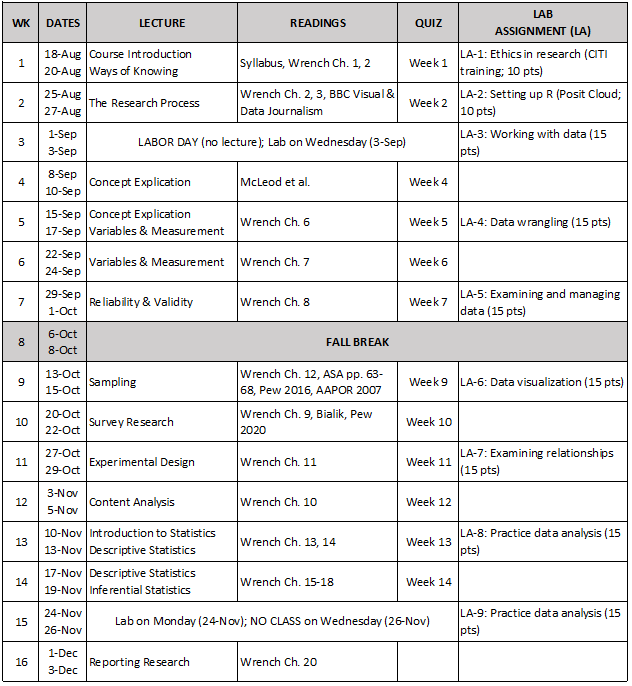
\includegraphics[keepaspectratio]{3710-schedule-F2025.png}}




\end{document}
